% Appendix B
\chapter{Additional figures}
\label{appendix:figures} % For referencing this appendix elsewhere, use \ref{AppendixA}

\lhead{Appendix C. \emph{Additional figures}} % This is for the header on each page - perhaps a shortened title

\begin{comment}
\section{Scatter plots for \dten}
\begin{figure}
\centering
\includegraphics[width=0.7\textwidth]{103_scatter_manual_outlier/d10/d.png}
\caption{Scatter plot of $\log \stdev$, $\log \roundstable$ and \timetoreachnewfundamental}
\end{figure}

\begin{figure}
\centering
\includegraphics[width=0.7\textwidth]{103_scatter_manual_outlier/d10/l.png}
\caption{Scatter plot of $\log \stdev$, $\log \roundstable$ and \overshoot}
\end{figure}

\begin{figure}
\centering
\includegraphics[width=0.7\textwidth]{103_scatter_manual_outlier/d10/f.png}
\caption{Scatter plot of \roundstable, \timetoreachnewfundamental and \stdev}
\end{figure}
\begin{figure}
\centering
\includegraphics[width=0.7\textwidth]{103_scatter_manual_outlier/d10/j.png}
\caption{Scatter plot of \overshoot, $\log \roundstable$ and \timetoreachnewfundamental}
\end{figure}

\section{Correlation plots of \sclatencys and \ssmmlatencys}
\begin{figure}{!h}
	%issue 15
	\centering
	\subcaptionbox{Correlation between \sclatencymu and \overshoot}
	[0.49\linewidth]{\includegraphics[width=0.5\textwidth]{101_pars_vs_fits/d10/sc_latency_s__vs__overshoot(mean)_scatter.png}}
	\subcaptionbox{Correlation between \sclatencymu and \roundstable}
	[0.49\linewidth]{\includegraphics[width=0.5\textwidth]{101_pars_vs_fits/d10/sc_latency_s__vs__round_stable(mean)_scatter.png}}
	\subcaptionbox{Correlation between \sclatencymu and \stdev}
	[0.49\linewidth]{\includegraphics[width=0.5\textwidth]{101_pars_vs_fits/d10/sc_latency_s__vs__stdev(mean)_scatter.png}}
	\subcaptionbox{Correlation between \sclatencymu and \timetoreachnewfundamental}
	[0.49\linewidth]{\includegraphics[width=0.5\textwidth]{101_pars_vs_fits/d10/sc_latency_s__vs__time_to_reach_new_fundamental(mean)_scatter.png}}
	\caption{Correlation between \sclatencys{} and the four fitness measures in experiment \dten}

\end{figure}

\begin{figure}[!h]
	%issue 15
	\centering
	\subcaptionbox{Correlation between \sclatencymu and \overshoot}
	[0.49\linewidth]{\includegraphics[width=0.5\textwidth]{101_pars_vs_fits/d10/ssmm_latency_s__vs__overshoot(mean)_scatter.png}}
	\subcaptionbox{Correlation between \sclatencymu and \roundstable}
	[0.49\linewidth]{\includegraphics[width=0.5\textwidth]{101_pars_vs_fits/d10/ssmm_latency_s__vs__round_stable(mean)_scatter.png}}
	\subcaptionbox{Correlation between \sclatencymu and \stdev}
	[0.49\linewidth]{\includegraphics[width=0.5\textwidth]{101_pars_vs_fits/d10/ssmm_latency_s__vs__stdev(mean)_scatter.png}}
	\subcaptionbox{Correlation between \sclatencymu and \timetoreachnewfundamental}
	[0.49\linewidth]{\includegraphics[width=0.5\textwidth]{101_pars_vs_fits/d10/ssmm_latency_s__vs__time_to_reach_new_fundamental(mean)_scatter.png}}
	\caption{Correlation between \sclatencys{} and the four fitness measures in experiment \dten}
	
\end{figure}

\end{comment}


\begin{comment}
\section{Scatter plots for \deleven}
\begin{figure}
\centering
\includegraphics[width=0.7\textwidth]{103_scatter_manual_outlier/d11/d.png}
\caption{Scatter plot of $\log \stdev$, $\log \roundstable$ and \timetoreachnewfundamental}
\end{figure}

\begin{figure}
\centering
\includegraphics[width=0.7\textwidth]{103_scatter_manual_outlier/d11/l.png}
\caption{Scatter plot of $\log \stdev$, $\log \roundstable$ and \overshoot}
\end{figure}

\begin{figure}
\centering
\includegraphics[width=0.7\textwidth]{103_scatter_manual_outlier/d11/f.png}
\caption{Scatter plot of \roundstable, \timetoreachnewfundamental and \stdev}
\end{figure}
\begin{figure}
\centering
\includegraphics[width=0.7\textwidth]{103_scatter_manual_outlier/d11/j.png}
\caption{Scatter plot of \overshoot, $\log \roundstable$ and \timetoreachnewfundamental}
\end{figure}
\end{comment}
